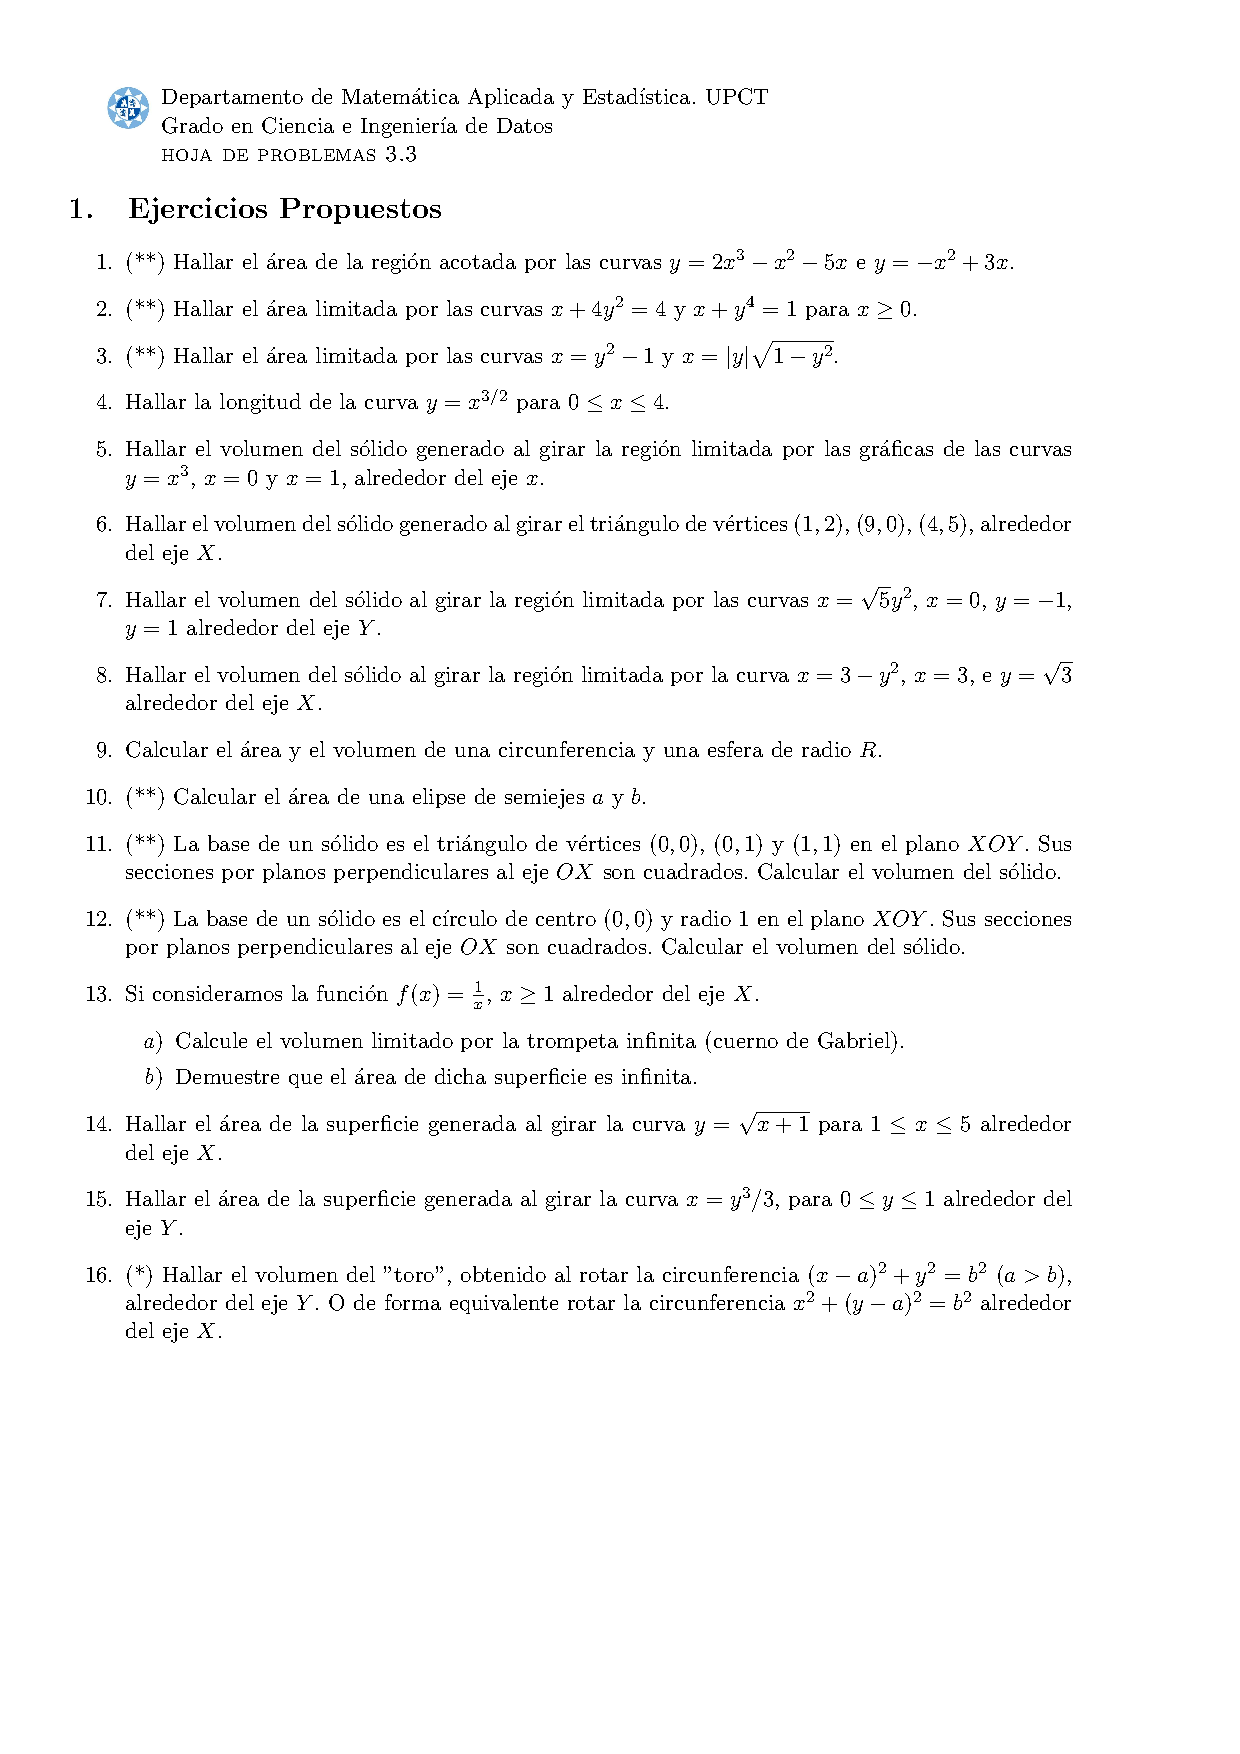
\includepdf[pages=-]{Tareas/Tema 3/Hoja 3.3/Hoja 3.3.pdf}

\begin{enumerate}[label=\color{red}\textbf{\arabic*)}, leftmargin=*]
	\item \lb{Hallar el área de la región acotada por las curvas $y=2x^3-x^2-5x$ e $y=-x^2+3x$.}
      
      $\begin{array}{l}
            \begin{rcases}
            y=2x^3-x^2-5x\\
            y=-x^2+3x
      \end{rcases}2x^3-\cancel{x^2}-5x=-\cancel{x^2}+3x\\
      \left|\int_{-2}^{0}2x^3-x^2-5-(-x^2+3x)\dx\right|+\left|\int_{0}^{2}2x^3-x^2-5-(x^2+3x)\dx\right|
      \end{array}$
      
	\item \lb{Hallar el área limitada por la curvas $x+4y^2=4$ y $x+y^4=1$ para $x\ge0$.}
      
      $\begin{array}{l}
            \begin{array}{ll}
                  \lb{1)} & x+4y^2=4\\
                  \lb{2)} & x+y^4=1\longrightarrow x=1-y^4
            \end{array}\quad x\ge0\\
            x=4-4y^2\longrightarrow x=4-4\cdot3=4-12=-8\\
            \lb{1)}\longrightarrow y=\pm\sqrt{\dfrac{4-x}{4}}\qquad\begin{array}{l}
                  4-4y^2=1-y^4\\
                  3-4y^2+y^4=0
            \end{array}\\
            y^4-4y^2+3=0\\
            y^2=\dfrac{4\pm\sqrt{(-4)^2-4\cdot1\cdot3}}{2}=\dfrac{4\pm\sqrt{16-12}}{2}=\left\langle\begin{array}{l}
                  \dfrac{4+2}{2}=3\left\langle\begin{array}{l}
                        \xcancel{\sqrt{3}}\\
                        \xcancel{-\sqrt{3}}
                  \end{array}\right. \\
                  \dfrac{4-2}{2}=1\left\langle\begin{array}{l}
                        1\\
                        -1
                  \end{array}\right.
            \end{array}\right. 
      \end{array}$
	\item \lb{Hallar el área limitada por las curvas $x=y^2-1$ y $x=|y|\sqrt{1-y^2}$.}
      
      $\begin{array}{l}
            x=y^2-1 \\
            x=|y|\sqrt{1-y^2}\\
            y^2-1=|y|\sqrt{1-y^2}\\
            y^4+1-2y^2=y(1-y^2)\\
            y^4+1+2y^2=y-y^3\\
            y^4+y^3-2y^2y+1=0\\
            2\cdot\left|\int_{0}^{1}(y^2-1)-y\sqrt{1y^2}\dy\right|
      \end{array}$
	\item \lb{Hallar la longitud de la curva $y=x^{\frac{3}{2}}$ para $0\le x\le4$.}
	\item \lb{Hallar el volumen del sólido generado al girar la región limitada por las gráficas de las curvas $y=x^3,\:x=0$ y $x=1$, alrededor del eje $x$.}
	\item \lb{Hallar el volumen del sólido generado al girar el triángulo de vértices (1,2), (9,0), (4,5), alrededor del eje $X$.}
	\item \lb{Hallar el volumen del sólido al girar la región limitada por las curvas $x=\sqrt{5}y^2,\:x=0,\:y=-1,\:y=1$ alrededor del eje $Y$.}
	\item \lb{Hallar el volumen del sólido al girar la región limitada por la curva $x=3-y^2,\:x=3,$ e $y=\sqrt{3}$ alrededor del eje $X$.}
	\item \lb{Calcular el área y el volumen de una circunferencia y una esfera de radio $R$.}
	\item \lb{Calcular el área de una elipse de semiejes $a$ y $b$.}
	\item \lb{La base de un sólido es el triángulo de vértices (0,0), (0,1) y (1,1) en el plano $XOY$. Sus secciones por planos perpendiculares al eje $OX$ son cuadrados. Calcular el volumen del sólido.}
	\item \lb{La base de un sólido es el círculo de centro (0,0) y radio 1 en el plano $XOY$. Sus secciones por planos perpendiculares al eje $OX$ son cuadrados. Calcular el volumen del sólido.}
	\item \lb{Si consideramos la función $f(x)=\dfrac{1}{x},\:x\ge1$ alrededor del eje $X$.}
	\begin{enumerate}[label=\color{red}\alph*)]
		\item \db{Calcule el volumen limitado por la trompeta infinita (cuerno de Gabriel).}
		\item \db{Demuestre que el área de dicha superficie es infinita.}
	\end{enumerate}
	\item \lb{Hallar el área de la superficie generada al girar la curva $y=\sqrt{x+1}$ para $1\le x\le 5$ alrededor del eje $X$}
	\item \lb{Hallar el área de la superficie generada al girar la curva $x=\dfrac{y^3}{3}$, para $0\le y\le1$ alrededor del eje $Y$.}
	\item \lb{Hallar el volumen del ``toro'', obtenido al rotar la circunferencia $(x-a)^2+y^2=b^2\:(a>b)$, alrededor del eje $Y$. O de forma equivalente rotar la circunferencia $x^2+(y-a)^2=b^2$ alrededor del eje $X$.}
\end{enumerate}